\documentclass[onecolumn,notitlepage,letterpaper,aps,pra,12pt]{article}
\usepackage[utf8]{inputenc}
\usepackage[spanish, es-tabla]{babel}
\usepackage[T1]{fontenc}
\usepackage[version=3]{mhchem}
\usepackage{titlesec}
\usepackage{enumitem}
\usepackage{pdfpages}
\usepackage{setspace}  
\usepackage{lmodern}
\usepackage{beamerarticle}
%\usepackage{multicol}
\usepackage{fancyhdr}
\setlength{\headheight}{15.13202pt}
\usepackage{graphics}
\usepackage{graphicx}
\usepackage{microtype} 
%\usepackage{natbib}
\usepackage[backend=bibtex,style=phys,natbib=true]{biblatex}

% Redefinimos el formato de los números en la bibliografía
\DeclareFieldFormat{labelnumberwidth}{[#1]} % Cambia superíndices a corchetes
\setlength{\biblabelsep}{0.5em} % Espacio entre el número y la referencia

\addbibresource{references.bib}
\DeclareFieldFormat[article]{title}{#1}
\usepackage{subfigure}
\usepackage{svg}
\usepackage{multirow} 
\usepackage{amssymb, amsmath, amsbsy} % simbolitos
\numberwithin{equation}{section}
\usepackage{upgreek} % para poner letras griegas sin cursiva
\usepackage{cancel} % para tachar
\usepackage{mathdots} % para el comando \iddots
\usepackage{mathrsfs} % para formato de letra
\usepackage{geometry}
\geometry{
	a4paper,
	total={150mm,257mm},
	left=20mm,
	top=20mm,
}
%\titleformat*{\section}{\bfseries\large}
%\titleformat*{\subsection}{\bfseries\normalsize}
\titleformat*{\section}{\normalfont\Large\bfseries\color{darkgray}}
\titleformat*{\subsection}{\normalfont\large\bfseries\color{gray}}
\titleformat*{\subsubsection}{\normalfont\normalsize\bfseries\color{blue}}
\usepackage{fancyhdr}
\pagestyle{fancy}
\rfoot{PROPUESTA DE INVESTIGACIÓN}
\renewcommand{\headrulewidth}{3pt}
\usepackage{tabularx}
\usepackage{supertabular}
\usepackage{vmargin}
\usepackage{mathtools} 
\usepackage{amsfonts}
\usepackage{float}
\usepackage{parskip}
\usepackage{times}
\usepackage{calligra}
\usepackage{latexsym}
\usepackage{booktabs}
\usepackage{tabulary}
\usepackage{caption}
\usepackage{url}
\spanishdecimal{.}
\usepackage{ragged2e}
%\bibliographystyle{unsrt}
\usepackage[usenames,dvipsnames]{pstricks}
\usepackage{epsfig}
\usepackage{pst-grad} % For gradients
\usepackage{pst-plot} % For axes
\usepackage{colortbl}
\usepackage{hyperref}
\usepackage{latexsym}
\usepackage{xcolor}
\usepackage{fancyhdr}
\usepackage{balance}
\usepackage{float}
\usepackage{bbold}
\usepackage[normalem]{ulem}
\usepackage{physics}
\usepackage{derivative}
\usepackage{tcolorbox}
\usepackage{amssymb}

% New commands
\newcommand{\miguel}[1]{{\color{magenta}#1}} 
\newcommand{\ricardo}[1]{{\color{red}#1}} 

%%%%%%%%%%%%%%%%%%%%%%%%%%%%%%
%%%%%%%%%%%%%%%%%%%%%%%%%%%%%%
\begin{document} 
%%%%%%%%%%%%%%%%%%%%%%%%%%%%%%
%%%%%%%%%%%%%%%%%%%%%%%%%%%%%%

\clearpage
\thispagestyle{empty}

%%%%%%%%%%%%%%%%%%%%%%%%%%%%%%
%%%%%%%%%%%%%%%%%%%%%%%%%%%%%%
\begin{titlepage}
\centering
\begin{figure}
    \centering
    
\includegraphics[width=4.5 in]{Images/uam.png}
\end{figure}

\vspace{1cm}

{\LARGE \rule{15cm}{1.0mm}  \par}

\centering
\vspace{0.45cm}

{\LARGE División de Ciencias Básicas e Ingeniería}

\centering
\vspace{0.45cm}

{\LARGE Posgrado en Ciencias (Física)}

\centering
\vspace{0.45cm}

{\LARGE Propuesta de Investigación Doctoral}

\vspace{0.25cm}

{\Huge \textbf{Fenómenos fuera de equilibrio en sistemas multimodo espín-bosón}}

\vspace{0.45cm}
{\large Propuesto por: {\bf M. en C. Ricardo Herrera Romero} \par}

\vspace{0.45cm}
{\large Matrícula: {\bf 2221801209} \par}

\vspace{0.45cm}
{\large Para sustentar el {\bf Examen Predoctoral} \par}

\vspace{0.45cm}
{\large Asesor: \textbf{Dr. Miguel Angel Bastarrachea Magnani}  \par}

\vspace{1cm}
\rule{5cm}{0.3mm}

\vspace{0.45cm}
{\large Coordinador: \textbf{Dr. Orlando Guzmán López}  \par}

{\LARGE \rule{15cm}{1.0mm}  \par}

\vspace{0.4cm}

{\large 18 de marzo de 2025 \par}
\vspace{0.1cm}
{\large Iztapalapa, Ciudad de México \par}
\end{titlepage}

%%%%%%%%%%%%%%%%%%%%%%%%%%%%%%
%%%%%%%%%%%%%%%%%%%%%%%%%%%%%%
\clearpage
\tableofcontents
\clearpage
\newpage
%%%%%%%%%%%%%%%%%%%%%%%%%%%%%%
%%%%%%%%%%%%%%%%%%%%%%%%%%%%%%

%%%%%%%%%%%%%%%%%%%%%%%%%%%%%%
%%%%%%%%%%%%%%%%%%%%%%%%%%%%%%
%\section*{Resumen}
%%%%%%%%%%%%%%%%%%%%%%%%%%%%%%
%%%%%%%%%%%%%%%%%%%%%%%%%%%%%%

%%%%%%%%%%%%%%%%%%%%%%%%%%%%%%
%%%%%%%%%%%%%%%%%%%%%%%%%%%%%%

%%%%%%%%%%%%%%%%%%%%%%%%%%%%%%
%%%%%%%%%%%%%%%%%%%%%%%%%%%%%%
\section{Introducción}
%%%%%%%%%%%%%%%%%%%%%%%%%%%%%%
%%%%%%%%%%%%%%%%%%%%%%%%%%%%%%



En las últimas décadas, los sistemas de interacción spin-bosón se han convertido en un área central en la física~\cite{haroche2006} CITAR. El desarrollo de plataformas experimentales como cavidades y circuitos en electrodinámica cuántica (\textit{Quantum Electrodynamics} o QED)~\cite{Blais2021,Clerk2020}, sistemas de átomos fríos~\cite{Mekhov2012}, trampas ópticas~\cite{Yuanjie2021} o semiconductores acoplados a microcavidades~\cite{Schneider2018}, han permitido explorar el acoplamiento controlado entre excitaciones bosónicas (fotones) y sistemas discretos de dos niveles (qubits o átomos de espin $1/2$). %Más allá de su interés en óptica cuántica, estas arquitecturas  funcionan como simuladores cuánticos de fenómenos colectivos~\cite{caballero2016}.

Los sistemas abiertos y fuertemente acoplados, donde la interacción entre spin-bosón es comparable o mayor que las frecuencias propias del sistema— han cobrado relevancia experimental en los últimos años~\cite{Grifoni1999,ZhangHou2015,Burger2022,Fazio2025}. La disipación y el bombeo generan estados de equilibrio dinámico con coherencia colectiva, que reflejan nuevas formas de comportamiento organizado~\cite{Sieberer2016,Halati2020,Chelpanova2025}. El interés se centra, por tanto, en la competencia entre coherencia, interacción spin-bosón y disipación, lo que permite comprender y controlar el comportamiento colectivo en regímenes de acoplamiento intenso~\cite{subasi2012,FornDiaz2019,Kirton2018,LeBoite2020,roses2020}.

Es en este marco conceptual modelos de spin-bosón como Rabi y Dicke adquieren relevancia, permitiendo analizar la dinámica de bombeo y disipación en estos sistemas~\cite{henriet2014,hwang2018,DiBello2024-2,Nagy10,Klinder15}. La propuesta de tesis doctoral se enmarca en esta dirección, con un enfoque sistemático y progresivo: comenzar con el modelo de Rabi abierto y avanzar hacia el modelo de Dicke abierto, incorporando tanto múltiples qubits como múltiples modos bosó\-nicos, para explorar la interacción colectiva y multimodal en presencia de bombeo y disipación.


%%%%%%%%%%%%%%%%%%%%%%%%%%%%%%
%%%%%%%%%%%%%%%%%%%%%%%%%%%%%%
\subsection{Modelos de interacción espín-bosón}
%%%%%%%%%%%%%%%%%%%%%%%%%%%%%%
%%%%%%%%%%%%%%%%%%%%%%%%%%%%%%

El estudio de la interacción entre la radiación y sistemas de dos niveles (espín–bosón) tiene su origen en el modelo de Rabi, propuesto para describir el acoplamiento coherente entre un átomo y un modo del campo electromagnético~\cite{rabi1936}. Su Hamiltoniano,

\begin{gather}\label{Hamiltoniano de Rabi}
    \hat{H}_{\text{Rabi}} = \omega\hat{a}^{\dagger}\hat{a} + \frac{\omega_{0}}{2}\hat{\sigma}_{z} + g\left( \hat{\sigma}_{+} + \hat{\sigma}_{-} \right)\left( \hat{a}^{\dagger} + \hat{a} \right),
\end{gather}

describe la energía del campo (frecuencia $\omega$) y del átomo (frecuencia $\omega_{0}$). El parámetro $g$ caracteriza el acoplamiento entre ambos, mientras que los términos rotantes $(\hat{\sigma}_{-}\hat{a} + \hat{\sigma}_{+}\hat{a}^{\dagger})$ representan procesos que conservan el número de excitaciones: la emisión o absorción de un fotón acompañada de la desexcitación o excitación atómica.

El modelo de Jaynes–Cummings~\cite{Jaynes1963} se obtiene aplicando la aproximación de onda rotante (RWA), que descarta los términos contra–rotantes $(\hat{\sigma}_{+}\hat{a}^{\dagger} + \hat{\sigma}_{-}\hat{a})$ válidos sólo en el régimen de acoplamiento débil $(g \ll \omega,\omega_{0})$. Esta aproximación permitió una descripción analítica del intercambio coherente de energía entre el átomo y el campo~\cite{wallraff2004,Schoelkopf2008,devoret2013}. Sin embargo, los avances experimentales han permitido acceder a los regímenes ultrastrong $(g/\omega \gtrsim 0.1)$ y deep strong $(g/\omega \gtrsim 1)$, donde la RWA deja de ser válida~\cite{FornDiaz2019,Yoshihara2017}, y se requiere el modelo de Rabi completo.

Un paso natural para extender el modelo a sistemas multiqubit consiste en analizar el caso de dos qubits acoplados colectivamente a un modo del campo, descrito por:

\begin{gather}
    \hat{H} = \omega\hat{a}^{\dagger}\hat{a} + \frac{\omega_{01}}{2}\hat{\sigma}_{z}^{1} + \frac{\omega_{02}}{2}\hat{\sigma}_{z}^{2} + \frac{g}{2}\left(\hat{\sigma}_{x}^{1}+\hat{\sigma}_{x}^{2}\right)(\hat{a}^{\dagger}+\hat{a}).
\end{gather}

Mediante los coeficientes de Clebsch–Gordan, los estados de los dos qubits pueden representarse en la base de espín total \( |J,M\rangle \), que se descompone en un subespacio simétrico triplete (\(J=1\)) y un singlete antisimétrico (\(J=0\)). Si las frecuencias atómicas son similares \(\omega_{01} \approx \omega_{02}\), el sistema es invariante bajo permutación y puede describirse dentro del subespacio simétrico \(J=1\). En esta representación, los operadores individuales se reemplazan por operadores colectivos \(\hat{J}_{\alpha}=\tfrac{1}{2}(\hat{\sigma}_{\alpha}^{1}+\hat{\sigma}_{\alpha}^{2})\), obteniendo el Hamiltoniano efectivo:

\begin{gather}\label{Hamiltoniano de Rabi dos qubits con interacciones}
    \hat{H} = \omega \hat{a}^{\dagger}\hat{a} + \omega_{0} \hat{J}_{z} + g \hat{J}_{x} (\hat{a}^{\dagger} + \hat{a}) + \eta_{x} \hat{J}_{x}^{2} + \eta_{z} \hat{J}_{z}^{2}.
\end{gather}

Los términos \(\eta_{z}\hat{J}_{z}^{2}\) y \(\eta_{x}\hat{J}_{x}^{2}\) introducen interacciones efectivas entre los qubits. El primero corresponde a un acoplamiento tipo Ising, que modula la energía según la alineación de los momentos atómicos; el segundo, de tipo XY, describe el intercambio coherente de excitaciones responsable de la correlación dinámica entre los emisores.

La generalización a un número arbitrario de átomos lleva al modelo de Dicke~\cite{Dicke54}, que describe la interacción colectiva entre $N$ átomos idénticos y un modo del campo electromagnético:

\begin{gather}
    \hat{H}_{\text{D}} = \omega\hat{a}^{\dagger}\hat{a} + \sum_{j=1}^{N}\left[ \frac{\omega_{0}}{2}\hat{\sigma}_{z}^{j} + \frac{g}{\sqrt{N}}\hat{\sigma}_{x}^{j}\left(\hat{a}^{\dagger} + \hat{a}\right) \right].
\end{gather}

Bajo la aproximación de onda larga~\cite{Dicke54}, todos los átomos experimentan el mismo campo, y el sistema puede describirse mediante los operadores de pseudospín colectivos \(\hat{J}_{\mu} = \frac{1}{2}\sum_{i=1}^{N}\hat{\sigma}_{\mu}^{i}\), lo que conduce a la forma compacta:

\begin{gather}\label{Dicke colectivo}
    \hat{H}_{\text{D}} = \omega\hat{a}^{\dagger}\hat{a} + \omega_{0}\hat{J}_{z} + \frac{2g}{\sqrt{N}}\hat{J}_{x}\left( \hat{a}^{\dagger} + \hat{a} \right).
\end{gather}

Este modelo predice fenómenos críticos como las transiciones de fase cuánticas (QPT) y las transiciones de fase cuánticas de estados excitados (ESQPT)~\cite{Hepp73,wang1973,hioe1973,Sachdev99,Larson17}. Cuando el acoplamiento luz-materia supera un valor crítico, el sistema pasa de un estado normal (sin fotones) a un estado superradiante caracterizado por emisión coherente colectiva~\cite{gross1982}. El modelo de Dicke ha sido implementado experimentalmente en diversas plataformas, como circuitos superconductores~\cite{Blais04,Casanova10} y cavidades ópticas con transiciones Raman~\cite{Baden14,Nagy10}, y se ha consolidado como un marco relevante en información cuántica~\cite{Garraway2011,Kirton2018,LeBoite2020}.



La inclusión de interacciones entre los átomos en el modelo de Dicke permite explorar nuevas fases y modificar los puntos críticos del sistema. En mi trabajo de maestría, estudié un modelo de Dicke anisotrópico con interacciones colectivas entre emisores, analizando su diagrama de fases y la aparición de QPT y ESQPT~\cite{Herrera2022}. Posteriormente identifiqué modos de fase y amplitud, relacionando anisotropía y criticidad en sistemas luz-materia fuertemente acoplados~\cite{herrera2024}. El Hamiltoniano correspondiente es:

\begin{gather}\label{Hamiltoniano de Dicke con interacciones}
    \hat{H}_{\text{I}} = \omega\hat{a}^{\dagger}\hat{a} + \omega_{0}\hat{J}_{z} + \frac{\gamma}{\sqrt{N}}\left[ \hat{a}\hat{J}_{+} + \hat{a}^{\dagger}\hat{J}_{-} + \xi\left( \hat{a}\hat{J}_{-} + \hat{a}^{\dagger}\hat{J}_{+} \right)  \right] + \frac{1}{N}\sum_{i=x,y,z} \eta_{i}\hat{J}_{i}^{2}.
\end{gather}

Los términos rotantes $(\hat{a}\hat{J}_{+}, \hat{a}^{\dagger}\hat{J}_{-})$ y contra–rotantes $(\hat{a}\hat{J}_{-}, \hat{a}^{\dagger}\hat{J}_{+})$ son modulados por el parámetro anisotrópico $\xi$, mientras que los términos $\eta_{i}$ cuantifican la interacción entre emisores.

Recientemente, se han propuesto extensiones multimodo del modelo de Dicke~\cite{tolkunov2007,fiorelli2020,carollo2021}, donde múltiples modos del campo electromagnético interactúan con los átomos:

\begin{gather}
        \hat{H}_{\text{Multimodo}} = \sum_{k}\left(\omega_{k}\hat{a}^{\dagger}_{k}\hat{a}_{k} + \sum_{j=1}^{N}\left[ \frac{\omega_{0}}{2}\hat{\sigma}_{z}^{j} + \sum_{k}\frac{g_{k}}{\sqrt{N}}\hat{\sigma}_{x}^{j}\left(\hat{a}^{\dagger}_{k} + \hat{a}_{k}\right) \right]\right).
\end{gather}

Estos sistemas presentan fenómenos como competencia entre modos, fases no convencionales y efectos de desorden~\cite{rotondo2015,kipf2014,vojta2013,das2024}, con implicaciones en el almacenamiento cuántico y redes neuronales cuánticas~\cite{maniscalco2006,fiorelli2020,marsch2021}.

De manera paralela, la física de los llamados “átomos gigantes” ha emergido como una extensión natural de estos modelos. En ellos, un solo emisor se acopla a un campo en múltiples puntos espaciales, generando retardos, interferencias y efectos no markovianos~\cite{Andersson2019,gonzalez2021-2,cai2021,yu2025}. Su tamaño efectivo, comparable con la longitud de onda del campo, rompe la aproximación dipolar y permite fenómenos como estados ligados dentro y fuera del continuo (BIC y BOC)~\cite{gonzalez2025,guo2020}. Experimentalmente, estos sistemas se implementan en circuitos superconductores donde qubits tipo transmon se acoplan en múltiples puntos de una guía de onda~\cite{Kannan2020}.

Los átomos gigantes constituyen un puente entre los modelos multiqubit y multimodo, donde la estructura espacial y temporal del acoplamiento genera nuevas dinámicas colectivas. Su estudio abre oportunidades para comprender efectos de memoria cuántica y explorar arquitecturas de simulación cuántica con acoplamientos no markovianos. Esta línea se alinea con el enfoque progresivo de esta tesis: analizar cómo la inclusión de grados de libertad multiqubit y multifrecuencia bosónica en sistemas espín–bosón modifica la dinámica colectiva y ofrece nuevas oportunidades para la simulación y las tecnologías cuánticas.


%%%%%%%%%%%%%%%%%%%%%%%%%%%%%%
%%%%%%%%%%%%%%%%%%%%%%%%%%%%%%
\subsection{Sistemas abiertos y dinámica fuera del equilibrio}
%%%%%%%%%%%%%%%%%%%%%%%%%%%%%%
%%%%%%%%%%%%%%%%%%%%%%%%%%%%%%

La física de sistemas cuánticos abiertos proporciona el marco teórico esencial para describir sistemas reales que interactúan con su entorno, desde átomos fríos y condensados de Bose–Einstein hasta circuitos superconductores y plataformas de óptica cuántica~\cite{rotter2015}. A diferencia de los sistemas cerrados, cuya evolución es puramente unitaria, los sistemas abiertos presentan disipación, ruido y pérdida de coherencia debido al acoplamiento con grados de libertad externos~\cite{Sieberer2016,breuer2003}.

En estos sistemas, el intercambio de energía con el entorno puede ser de dos tipos: el bombeo coherente, que permite transferencia controlada de energía preservando coherencia cuántica, y el bombeo incoherente, de origen térmico o aleatorio, que introduce ruido y degradación de información~\cite{carmichael2013}. Esta dualidad permite estudiar cómo coherencia y disipación compiten o cooperan para generar dinámicas estacionarias fuera del equilibrio.

La evolución temporal se describe mediante ecuaciones maestras para el operador densidad. La ecuación de Linblald incorpora sistemáticamente procesos de disipación y bombeo, llevando a estados estacionarios que no corresponden a estados térmicos, sino a configuraciones mantenidas por flujos continuos de energía~\cite{Li2014,Fazio2025}. Complementariamente, el formalismo de Keldysh ofrece una formulación de campo fuera del equilibrio que unifica coherencia y disipación en un marco de acción efectiva~\cite{Sieberer2016,chakraborty2018}.

Estas herramientas teóricas han sido cruciales para describir la competencia entre coherencia, interacción y pérdida en plataformas experimentales como cavidades ópticas~\cite{torres2013}, circuitos superconductores~\cite{feigelman2000} y condensados de polaritones~\cite{dunnet2016}. En el contexto de esta tesis, permiten abordar sistemáticamente los regímenes de bombeo y disipación en modelos de interacción luz-materia, desde el modelo de Rabi abierto hasta extensiones multimodo y sistemas con átomos gigantes.

%%%%%%%%%%%%%%%%%%%%%%%%%%%%%%
%%%%%%%%%%%%%%%%%%%%%%%%%%%%%%
\subsection{Modelo de Rabi y Dicke abierto}
%%%%%%%%%%%%%%%%%%%%%%%%%%%%%%
%%%%%%%%%%%%%%%%%%%%%%%%%%%%%%

Los modelos de Rabi y Dicke proporcionan el marco teórico para estudiar sistemas abiertos con disipación~\cite{henriet2014,hwang2018,zueco2019,Lyu2024,damanet2019,Grimsmo2013}. En el modelo de Rabi abierto emerge una transición de fase disipativa de segundo orden, donde la competencia entre acoplamiento ultrastrong y disipación conduce a un estado estacionario con incremento significativo de excitaciones, incluso en sistemas pequeños~\cite{hwang2018}.

El modelo de Dicke abierto incorpora explícitamente disipación (pérdida de fotones y relajación atómica) y bombeo externo, dando lugar a transiciones de fase dinámicas~\cite{kirton2017,LeBoite2020} como oscilaciones coherentes sostenidas~\cite{mivehvar2021} y cristales de tiempo~\cite{zhu2019}.

\begin{figure}[H]
    \centering
    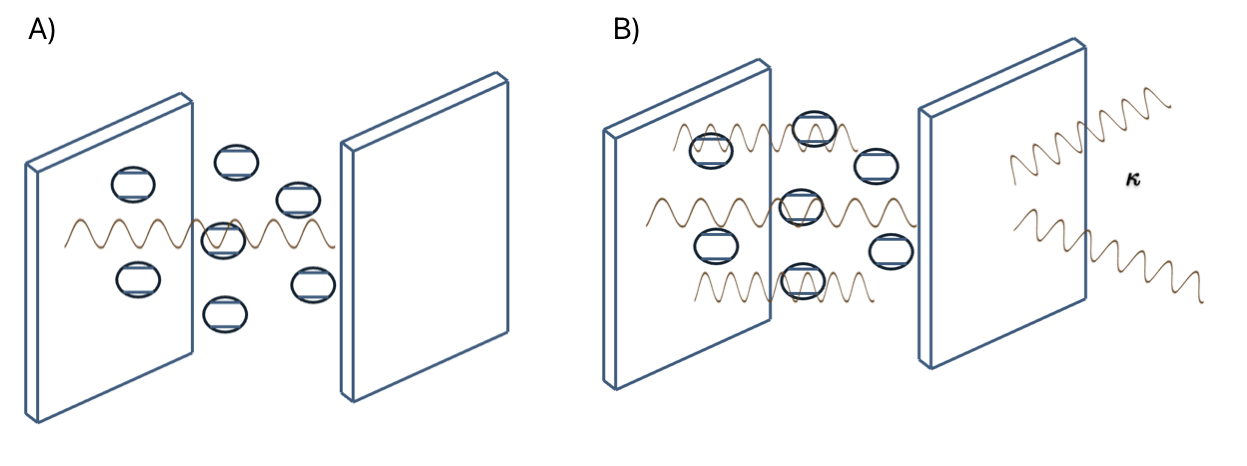
\includegraphics[width=0.9\linewidth]{Images/cavity1.png}
    \caption{Ilustración del modelo de Dicke. 
A) \( N \) átomos de dos niveles interactúan con un único modo electromagnético. 
B) \( N \) átomos interactúan con múltiples modos, incorporando bombeo y disipación \( \kappa \).}
    \label{Figure Cavity}
\end{figure}

La primera observación experimental de la transición superradiante fue realizada por Baumann et al.~\cite{Baumann11} acoplando un condensado de Bose–Einstein (BEC) a una cavidad óptica abierta. Este experimento reveló la ruptura espontánea de simetría durante la transición, mostrando cómo las fluctuaciones cuánticas y efectos disipativos compiten en regímenes fuera del equilibrio~\cite{Baumann10}. Experimentos posteriores con BEC en cavidades ópticas demostraron que la transición superradiante puede mantenerse en régimen no térmico~\cite{Baumann10,Klinder15}, mientras que en circuitos QED se observaron dinámicas colectivas estacionarias inducidas por disipación~\cite{Blais2021}. Estos resultados establecieron la disipación como elemento activo para generar y estabilizar orden cuántico colectivo.

Los sistemas optomecánicos~\cite{debnath2015} y los qubits superconductores~\cite{Lamata2017} han emergido como plataformas experimentales clave. Los primeros permiten estudiar acoplamientos entre modos ópticos y mecánicos, mientras que los segundos ofrecen control preciso sobre parámetros fundamentales, facilitando la exploración experimental de los modelos de Rabi y Dicke~\cite{Mezzacapo14} y su interacción con el entorno~\cite{hwang2018,Lo2021}.

Recientemente, el modelo de Dicke multimodo en regímenes fuera de equilibrio ha mostrado comportamientos análogos a memorias asociativas, con capacidad de reconocer patrones almacenados~\cite{fiorelli2020}. Más allá del régimen Markoviano, sistemas no-Markovianos como los átomos gigantes —donde un emisor se acopla al campo en múltiples puntos espaciales— introducen retardos y correlaciones temporales que permiten simular interacciones con memoria~\cite{kockum2019,guo2020}. Estas configuraciones consolidan el \textit{reservoir engineering} como técnica para diseñar entornos que protegen o inducen coherencia, estabilizando estados coherentes y entrelazados~\cite{poyatos1996,Diehl2008}.


%%%%%%%%%%%%%%%%%%%%%%%%%%%%%%
%%%%%%%%%%%%%%%%%%%%%%%%%%%%%%
\subsection{Conclusión}
%%%%%%%%%%%%%%%%%%%%%%%%%%%%%%
%%%%%%%%%%%%%%%%%%%%%%%%%%%%%%

Este proyecto de investigación doctoral tiene como objetivo principal estudiar sistemáticamente los modelos de Rabi y Dicke en regímenes multimodo y multiqubit, con especial énfasis en sistemas abiertos y fuera de equilibrio. La investigación se estructura progresivamente, comenzando con el modelo de Rabi de dos qubits, sistemas de multifrecuencia bosónica como los átomos gigantes y  avanzando hacia configuraciones colectivas más complejas del modelo de Dicke  donde los efectos no-Markovianos y la estructura  extendida enriquecen sustancialmente la dinámica.



%%%%%%%%%%%%%%%%%%%%%%%%%%%%%%
%%%%%%%%%%%%%%%%%%%%%%%%%%%%%%
\section{Objetivos}
%%%%%%%%%%%%%%%%%%%%%%%%%%%%%%
%%%%%%%%%%%%%%%%%%%%%%%%%%%%%%

\subsection{Objetivo general}

El objetivo central de esta investigación doctoral es establecer un marco teórico para comprender la dinámica colectiva en sistemas cuánticos abiertos con interacción luz-materia en regímenes de acoplamiento intenso, multimodo y multiqubit. Buscamos describir cómo la competencia entre coherencia, disipación y bombeo externo genera nuevas fases cuánticas fuera del equilibrio, con relevancia tanto para la física fundamental como para el desarrollo de tecnologías cuánticas.

Este objetivo se aborda progresivamente, desde modelos de baja dimensionalidad —como el de Rabi extendido con interacciones entre qubits— hasta configuraciones colectivas del modelo de Dicke abierto y multimodo. El hilo conductor será identificar los mecanismos que permiten la emergencia de orden cuántico en presencia de disipación, memoria y acoplamientos espaciales no triviales, como los presentes en sistemas con átomos gigantes.

\subsection{Objetivos específicos}

\begin{itemize}
    \item Analizar el modelo de Rabi de dos qubits con interacciones materiales, Eq.~\eqref{Hamiltoniano de Rabi dos qubits con interacciones} y caracterizar como la inclusión de términos de un qubit e interacciones materiales modifican el espectro de energía. Este estudio servirá como base conceptual para entender el acoplamiento colectivo entre múltiples emisores.
    
    \item Estudiar configuraciones de átomos gigantes, para entender fenómenos no markovianos, analizando los retardos y correlaciones temporales inducidos por el entorno, así como su impacto sobre la coherencia y la memoria cuántica para posibles aplicaciones en Rabi y Dicke.
    

    \item Desarrollar una descripción teórica del modelo de Rabi abierto incorporando disipación y bombeo en el marco de la ecuación maestra de Lindblad, con el fin de identificar regímenes estacionarios fuera del equilibrio y la posible aparición de transiciones disipativas.

    \item Extender el análisis al modelo de Dicke multiqubit, investigando cómo los emisores afectan las transiciones superradiantes, las propiedades críticas del sistema y la estructura de fases cuánticas de equilibrio y no equilibrio.

    \item Explorar el modelo de Dicke multimodo abierto, utilizando el formalismo de Keldysh para describir la competencia entre múltiples modos bosónicos, el bombeo incoherente y la disipación, con especial atención a la emergencia de oscilaciones coherentes sostenidas y cristales de tiempo.

    

    %\item \textbf{Proponer un marco general para la ingeniería de entornos cuánticos} (\textit{reservoir engineering}) que permita diseñar o controlar estados colectivos estacionarios, con potencial aplicación en simuladores cuánticos, procesamiento de información y almacenamiento coherente de excitaciones.

\end{itemize}



%%%%%%%%%%%%%%%%%%%%%%%%%%%%%%
%%%%%%%%%%%%%%%%%%%%%%%%%%%%%%
\section{Metodología}
%%%%%%%%%%%%%%%%%%%%%%%%%%%%%%
%%%%%%%%%%%%%%%%%%%%%%%%%%%%%%

Esta sección presenta el marco metodológico para abordar los primeros objetivos de esta propuesta doctoral. El planteamiento se estructura en dos partes:  el estudio del modelo de Rabi extendido a dos qubits con interacciones materiales, como primer acercamiento a sistemas multiqubit; y el análisis de átomos gigantes en guías de onda estructuradas, que permiten explorar fenómenos multimodales bosónicos y efectos no markovianos. 

%%%%%%%%%%%%%%%%%%%%%%%%%%%%%%
%%%%%%%%%%%%%%%%%%%%%%%%%%%%%%
\subsection{Modelo de Rabi de dos qubits con interacciones materiales}
%%%%%%%%%%%%%%%%%%%%%%%%%%%%%%
%%%%%%%%%%%%%%%%%%%%%%%%%%%%%%

Este estudio sistemático del modelo de Rabi con dos qubits e interacciones materiales constituye un primer paso hacia la comprensión de sistemas multiqubit. El objetivo es analizar cómo la incorporación de un segundo qubit y la presencia de interacciones materiales modifican el espectro energético y los estados propios del sistema.

Con este propósito, se implementan tres aproximaciones  que nos permiten realizar futuras extensiones hacia sistemas con un mayor número de qubits, proporcionando un marco conceptual para explorar la evolución de la dinámica cuántica conforme se incrementa la complejidad del modelo.


%%%%%%%%%%%%%%%%%%%%%%%%%%%%%%
\subsubsection{Diagonalización numérica exacta}
%%%%%%%%%%%%%%%%%%%%%%%%%%%%%%

Como referencia, empleamos diagonalización numérica directa del Hamiltoniano~\eqref{Hamiltoniano de Rabi dos qubits con interacciones}, que proporciona resultados numéricamente exactos para validar nuestras aproximaciones analíticas. 

La elección del subespacio simétrico ($j=1$) constituye una simplificación física. Se justifica por la invariancia del Hamiltoniano bajo permutación de qubits idénticos ($\omega_{01} \approx \omega_{02}$), que confina la dinámica al sector triplete donde los operadores colectivos $\hat{J}_{\alpha} = \frac{1}{2}(\hat{\sigma}_{\alpha}^{1} + \hat{\sigma}_{\alpha}^{2})$ capturan completamente el comportamiento del sistema. Físicamente, esto significa que los qubits son indistinguibles y se comportan como una entidad colectiva. El singlete antisimétrico ($j=0$) permanece desacoplado tanto del campo como de las interacciones materiales, haciendo que no participen en la dinámica principal.

En la base producto $|\Psi\rangle = |n\rangle \otimes |j, m\rangle$ con $j=1$ y $m = -1, 0, 1$, los elementos de matriz adquieren una estructura físicamente transparente:

\small{ 
\begin{gather}
    \langle n', m' | \hat{H} | n, m \rangle 
    = \omega n\delta_{n',n} + \left(\omega_{0} + \eta_{z}m\right) m\delta_{m',m} 
    + \frac{g}{2}\left( \sqrt{n+1}\delta_{n',n+1} + \sqrt{n}\delta_{n',n-1} \right) \nonumber \\
    \times\left(\sqrt{j(j+1) - m(m+1)}\delta_{m',m+1} + \sqrt{j(j+1) - m(m-1)}\delta_{m',m-1}\right) \nonumber \\
    +\frac{\eta_{x}}{4}\left(\sqrt{j(j+1)-m(m+1)}\sqrt{j(j+1)-(m+1)(m+2)}\delta_{m',m+2} \right. \nonumber \\
    \left. +2\left(j(j+1) - m^{2}\right)\delta_{m',m} \right. \nonumber \\
    \left. +\sqrt{j(j+1) - m(m-1)}\sqrt{j(j+1)-(m-1)(m-2)}\delta_{m',m-2}\right) \label{numerica two qubit}
\end{gather}}   

Cada término tiene una interpretación física clara: el primer renglón describe las energías libres del oscilador y los qubits (modificada por $\eta_z$), el segundo captura el acoplamiento qubit-campo, y el tercero representa las interacciones materiales de tipo Ising ($\eta_z$) y XY ($\eta_x$).

%%%%%%%%%%%%%%%%%%%%%%%%%%%%%%
\subsubsection{Aproximación adiabática}
%%%%%%%%%%%%%%%%%%%%%%%%%%%%%%

Como primera aproximación analítica, consideramos el límite adiabático ($\omega_0 \rightarrow 0$), donde el oscilador se ajusta instantáneamente a la configuración de los qubits. Esta aproximación corresponde físicamente al régimen donde la frecuencia del oscilador domina sobre el desacople de los qubits, una situación común en sistemas de circuitos QED donde $\omega \gg \omega_0$.

La transformación $\hat{U} = \exp\left[{\beta(\hat{a}^{\dagger}-\hat{a})}\right]$ genera estados de Fock desplazados que describen el reacomodo del campo para cada configuración de qubits. Físicamente, podemos visualizar esto como si el campo electromagnético se ''adaptara'' instantáneamente a la orientación de los espines, creando pozos de potencial efectivos que dependen del estado de los qubits.

Esta aproximación conserva únicamente acoplamientos entre estados con el mismo número de excitaciones, resultando en un Hamiltoniano efectivo con estructura de bloques diagonales. Si bien proporciona una imagen física intuitiva y captura correctamente el estado fundamental, su limitación principal reside en ignorar completamente los efectos de tunelado cuántico ($\omega_0 \neq 0$), lo que lleva a discrepancias significativas en el espectro de excitaciones.

%%%%%%%%%%%%%%%%%%%%%%%%%%%%%%
\subsubsection{Aproximación de la onda rotante generalizada}
%%%%%%%%%%%%%%%%%%%%%%%%%%%%%%

La Aproximación Generalizada de Onda Rotante (\text{Generalized Rotating Wave Approximation} o GRWA)~\cite{irish2007,albert2011,yu2012,zhang2015,zhangyu2016,zhangyu2017}  extiende el enfoque adiabático reintroduciendo consistentemente el tunelado cuántico mediante una transformación polarónica:

\begin{gather}\label{transformation beta}
    \hat{U} = \exp\left[ \beta\hat{J}_{x}(\hat{a}^{\dagger} - \hat{a}) \right],
\end{gather}

con $\beta = g/\omega$ determinado variacionalmente mediante minimización de la energía del estado fundamental. Físicamente, esta transformación representa un desplazamiento colectivo del campo electromagnético que incorpora de manera autoconsistente la retroalimentación entre los qubits y el oscilador.

La potencia de la GRWA reside en que preserva la estructura de bloques manejable de la aproximación adiabática mientras incluye correcciones esenciales que permiten describir transiciones entre diferentes números de excitaciones. Matemáticamente, esto se logra mediante la resolución de un problema de valores propios en cada bloque del Hamiltoniano transformado, donde ahora se retienen acoplamientos cruciales que la aproximación adiabática descartaba.

Los resultados demuestran que la GRWA aproxima incluso regimenes de acoplamiento fuerte, capturando  tanto el estado fundamental como las excitaciones de baja energía. Esta robustez la convierte en una herramienta  para explorar regímenes de acoplamiento donde los métodos perturbativos convencionales fallan.

Esta metodología progresiva —desde la aproximación adiabática simple hasta la GRWA, validadas sistemáticamente contra resultados numéricos exactos— establece las bases conceptuales y técnicas para extender nuestro análisis a sistemas multiqubit más complejos.


%%%%%%%%%%%%%%%%%%%%%%%%%%%%%%
%%%%%%%%%%%%%%%%%%%%%%%%%%%%%%
\subsection{Átomos gigantes en guías de onda de arreglo de cavidades}
%%%%%%%%%%%%%%%%%%%%%%%%%%%%%%
%%%%%%%%%%%%%%%%%%%%%%%%%%%%%%

El estudio de átomos gigantes representa la segunda paso de nuestra metodología, extendiendo nuestro análisis hacia sistemas donde la estructura espacial extendida del emisor introduce fenómenos ricos en física no markoviana y efectos de interferencia, además ofrece una plataforma para explorar interacciones luz-materia en regímenes multimodales.

%%%%%%%%%%%%%%%%%%%%%%%%%%%%%%
\subsubsection{Modelo básico y transformada de Fourier}
%%%%%%%%%%%%%%%%%%%%%%%%%%%%%%

El punto de partida es un emisor de dos niveles acoplado a un arreglo unidimensional de cavidades, descrito por el Hamiltoniano:

\[H = \delta\sigma^{+}\sigma^{-} + \omega_{0}\sum_{n}a^{\dagger}_{n}a_{n} + \xi\sum_{n}\left(a^{\dagger}_{n+1}a_{n} + a^{\dagger}_{n}a_{n+1}\right) + g_{0}\left(\sigma^{+}a_{0} + \sigma^{-}a^{\dagger}_{0}\right).\]

La estrategia de solución aprovecha la invariancia traslacional del sistema mediante la transformación de Fourier discreta $a_{k} = N^{-1/2}\sum_{n}e^{ikn}a_{n}$. Esta transformación es fundamental pues diagonaliza la guía de onda, revelando la relación de dispersión $\omega_{k} = 2\xi\cos k$ que describe cómo se propagan los fotones a través del arreglo.

Físicamente, este cambio de perspectiva —de cavidades localizadas a modos extendidos— es crucial: en lugar de pensar en fotones saltando entre cavidades vecinas, trabajamos con modos colectivos que se propagan como ondas a lo largo de la guía. Esta representación nos permite describir procesos de emisión espontánea, donde un átomo excitado emite radiación que se propaga lejos del punto de emisión.

%%%%%%%%%%%%%%%%%%%%%%%%%%%%%%
\subsubsection{Función espectral}
%%%%%%%%%%%%%%%%%%%%%%%%%%%%%%

La función espectral $J(\omega) = \frac{2g_{0}^{2}}{\sqrt{4\xi^{2}-\omega^{2}}}$ emerge como una cantidad central que conecta la estructura de la guía de onda con la dinámica del emisor. Esta función captura cómo los diferentes modos de frecuencia $\omega$ contribuyen al acoplamiento efectivo con el emisor.

El comportamiento de $J(\omega)$ muestra lo siguiente: cerca del centro de la banda ($\omega \approx 0$), la función es aproximadamente constante, recuperando la dinámica markoviana tradicional con decadencia exponencial. Sin embargo, cerca de los bordes de banda ($\omega \approx \pm 2\xi$), las singularidades de van Hove indican el colapso de la aproximación markoviana y el surgimiento de dinámica altamente no markoviana.

Estas singularidades tienen consecuencias físicas profundas: representan un ralentizamiento crítico de la velocidad de grupo de los fotones, mostrando  una acumulación de densidad de estados que modifica cualitativamente la dinámica de emisión.

%%%%%%%%%%%%%%%%%%%%%%%%%%%%%%
\subsubsection{Transformada de Laplace}
%%%%%%%%%%%%%%%%%%%%%%%%%%%%%%

Para ir más allá de la aproximación de Weisskopf-Wigner, empleamos la transformada de Laplace, que permite descomponer analíticamente la solución temporal en contribuciones físicamente transparentes:

\[\alpha(t) = \lim_{\epsilon\to 0}\int_{-\omega_{\max}}^{-\omega_{\min}}\frac{dy}{2\pi}\frac{J(-y)e^{iyt}}{[y+\Delta-iG(-\epsilon+iy)]\,[y+\Delta-iG(\epsilon+iy)]} + \sum_{j}r_{j}e^{-iy_{j}t}.\]

Esta descomposición es notable: el primer término (integral sobre el corte de rama) representa la contribución de estados de scattering dentro del continuo, que eventualmente decaen a cero. El segundo término (suma sobre residuos) corresponde a estados ligados fuera del continuo (BOC) que persisten indefinidamente en el estado estacionario.

Físicamente, esta estructura explica por qué parte de la excitación inicial queda atrapada localmente alrededor del emisor, formando un estado ligado fotónico cuya función de onda decae exponencialmente con la distancia. La localización espacial de estos estados puede caracterizarse cuantitativamente mediante la longitud de localización $\lambda_{\pm} = \cosh^{-1} (|y_{\pm}|/2\xi)$.

%%%%%%%%%%%%%%%%%%%%%%%%%%%%%%
\subsubsection{Extensión a átomos gigantes}
%%%%%%%%%%%%%%%%%%%%%%%%%%%%%%

La generalización a átomos gigantes —donde un mismo emisor se acopla al campo en $N_c$ posiciones espacialmente separadas— introduce una capa adicional de riqueza física. El acoplamiento efectivo se modifica a:

\[\tilde{g}_k = \frac{g_0}{N_c\sqrt{N}} \frac{\sin(kdN_c/2)}{\sin(kd/2)},\]

donde $d$ es la separación entre puntos de acoplamiento.

Esta dependencia espacial modifica fundamentalmente la función espectral efectiva $J_{\text{eff}}(\omega) = J(\omega) \mathcal{G}(\omega)$, que ahora presenta ceros en frecuencias específicas $\omega_m = 2\xi\cos(\pi(2m+1)/d)$. En estas frecuencias, emergen estados ligados dentro del continuo (BIC) —estados que, contra-intuitivamente, están embebidos en el continuum pero no decaen.

El origen físico de los BIC reside en interferencia destructiva: las diferentes rutas que puede tomar un fotón emitido desde los distintos puntos de acoplamiento interfieren destructivamente, impidiendo que la radiación se escape al infinito. Estos estados confinan fotones en la región entre los puntos de acoplamiento, transformando efectivamente al átomo gigante en una cavidad óptica.



%%%%%%%%%%%%%%%%%%%%%%%%%%%%%%
%%%%%%%%%%%%%%%%%%%%%%%%%%%%%%
\subsection{Conclusión }
%%%%%%%%%%%%%%%%%%%%%%%%%%%%%%
%%%%%%%%%%%%%%%%%%%%%%%%%%%%%%

La metodología desarrollada establece un marco  progresivo para abordar los desafíos centrales de esta investigación doctoral. El estudio del modelo de Rabi de dos qubits con interacciones materiales provee las herramientas esenciales para comprender efectos colectivos en sistemas multiqubit, mientras que el análisis de átomos gigantes en guías de onda estructuradas permite explorar fenómenos no markovianos y multimodales.

Esta base metodológica no solo permite alcanzar los objetivos inmediatos de la tesis, sino que también habilita extensiones hacia sistemas con más qubits, geometrías complejas y dinámicas fuera del equilibrio con bombeo y disipación. Su versatilidad y coherencia la consolidan como una contribución relevante a las metodologías de investigación en óptica e información cuántica.


\section{Resultados esperados}

Esta investigación doctoral tiene como objetivo establecer un marco teórico para comprender los fenómenos colectivos en sistemas cuánticos abiertos, tanto multimodo como multiqubit. 

En una primera etapa, se abordará el estudio del modelo de Rabi con dos qubits acoplados y con interacciones materiales. El objetivo es caracterizar cómo la presencia de interacciones materiales entre qubits modifica el espectro energético del sistema. Se espera identificar patrones que puedan extenderse posteriormente a sistemas con mayor número de qubits. Para ello, se utilizarán distintas aproximaciones, desde métodos adiabáticos simples hasta la GRWA, comparándolas con resultados numéricos exactos.

En la línea de investigación sobre átomos gigantes, se extenderá el modelo hacia regímenes de acoplamiento fuerte, donde la interacción entre los emisores y el campo no puede tratarse como una perturbación débil. En estos sistemas, los estados excitados pueden formar \textit{estados ligados} dentro o fuera del continuo fotónico, lo que significa que el fotón puede quedar parcialmente confinado alrededor del átomo. La extensión espacial del emisor permite aprovechar efectos de interferencia para atrapar fotones en regiones específicas del espacio, generando cavidades ópticas ''virtuales''. 

Para describir la dinámica fuera del equilibrio en sistemas abiertos con interacciones fuertes, se empleará la teoría de Keldysh. Este formalismo extiende la teoría cuántica de campos (\textit{Quantum Field Theory}, QFT) al dominio del tiempo real mediante integrales de camino definidas sobre un contorno de Keldysh~\cite{kamenev2023,rammer2011}. A diferencia de los métodos tradicionales basados en ecuaciones maestras, la formulación de Keldysh permite tratar simultáneamente procesos coherentes (unitarios) y disipativos, capturando la evolución completa del sistema. Esto es especialmente útil para describir estados estacionarios no térmicos y analizar transiciones de fase en presencia de disipación y bombeo externo~\cite{Sieberer2016}.

De manera complementaria, se integrará la teoría del grupo de renormalización funcional (\textit{Functional Renormalization Group}, FRG), basada en la ecuación de Wetterich~\cite{wetterich1993}. Esta herramienta permite analizar la disipación a distintas escalas de energía y seguir la evolución del sistema desde sus interacciones microscópicas hasta comportamientos macroscópicos emergentes. La FRG resulta esencial en regímenes críticos, donde los métodos perturbativos fallan, ya que captura de manera no aproximada la competencia entre coherencia y disipación~\cite{angelakis2007}. Con ello, será posible estudiar la relajación hacia estados estacionarios y la formación de fases cuánticas no convencionales.

El estudio de sistemas abiertos también se abordará mediante la teoría de sistemas cuánticos disipativos, que describe cómo un sistema se acopla a su entorno. En la llamada aproximación markoviana, se asume que el entorno (o “baño”) no tiene memoria, de modo que los efectos de disipación ocurren instantáneamente. Bajo esta suposición, la evolución del sistema puede describirse mediante las ecuaciones maestras de Lindblad~\cite{breuer2003,Lindblad1976}, las cuales proporcionan una descripción efectiva ampliamente utilizada en óptica cuántica~\cite{weiss2012}.

Finalmente, se explorarán los efectos de memoria a largo plazo en sistemas de Dicke acoplados a baños no markovianos~\cite{zhu2019,lundgren2020,fiorelli2020}. En este caso, el entorno conserva información sobre su interacción previa con el sistema, generando correlaciones temporales que modifican la dinámica cuántica~\cite{orazio2016}. Este tipo de acoplamiento puede dar lugar a comportamientos ricos y no triviales, como oscilaciones persistentes o relajación no exponencial, y alterar la naturaleza de las transiciones de fase fuera del equilibrio~\cite{lundgren2020}.

Se espera que los resultados de esta investigación contribuyan al entendimiento del modelo de Dicke multimodo en presencia de disipación y bombeo, con énfasis en fenómenos como las transiciones de fase superradiantes, la competencia entre modos y los efectos del desorden o de las interacciones entre emisores. Asimismo, se buscará identificar nuevas fases fuera del equilibrio mediante el formalismo de Keldysh, incluyendo la posible formación de \textit{cristales de tiempo} y el desarrollo de memorias cuánticas con retención prolongada. En conjunto, estos avances ampliarán el conocimiento teórico sobre sistemas cuánticos abiertos y ofrecerán perspectivas aplicadas para el desarrollo de tecnologías cuánticas de próxima generación.


%%%%%%%%%%%%%%%%%%%%%%%%%%%%%%
%%%%%%%%%%%%%%%%%%%%%%%%%%%%%%
\section{Avances}
%%%%%%%%%%%%%%%%%%%%%%%%%%%%%%
%%%%%%%%%%%%%%%%%%%%%%%%%%%%%%


%%%%%%%%%%%%%%%%%%%%%%%%%%%%%%
\subsection{Modelo de Rabi de dos qubits con interacciones materiales}
%%%%%%%%%%%%%%%%%%%%%%%%%%%%%%

Mostramos algunos resultados del espectro de energías del modelo de Rabi de dos qubits con interacciones materiales utilizando la aproximación adiabática y GRWA. 

\subsubsection{Espectro energético y validación de la GRWA}

La validación sistemática de nuestras aproximaciones mediante diagonalización numérica exacta ($n_{\text{max}}=30$) revela que la Aproximación Generalizada de Onda Rotante (GRWA) aproxima el espectro del sistema. Como muestra la Figura~\ref{fig: Conventional GRWA}, la GRWA captura no solo la estructura general de niveles sino también detalles finos como curvaturas y cruces de niveles que emergen en el régimen de acoplamiento fuerte ($g/\omega \gtrsim 0.5$).

\begin{figure}[H]
    \centering
    \includegraphics[width=0.95\linewidth]{Images APS v1/GRWA.pdf}
    \caption{Espectro energético del modelo de Rabi de dos qubits. Las líneas negras sólidas representan la diagonalización numérica exacta. (a) Caso no resonante $\omega_0 = \omega/2$; (b) Caso resonante $\omega = \omega_0$; (c) Resonante con $\eta_z = 0.5$; (d) Resonante con $\eta_x = 0.5$. La GRWA (línea púrpura discontinua) muestra excelente acuerdo con los resultados exactos incluso en presencia de interacciones materiales.}
    \label{fig: Conventional GRWA}
\end{figure}

La robustez de la aproximación se mantiene al incorporar interacciones materiales $\eta_x$ y $\eta_z$, demostrando su versatilidad para describir sistemas donde los acoplamientos qubit-qubit modifican sustancialmente la dinámica luz-materia.

\subsubsection{Tratamiento variacional del estado fundamental}

Desarrollamos un enfoque variacional para optimizar la descripción del estado base. Partiendo de la transformación polarónica $\hat{U} = \exp\left[ \beta\hat{J}_{x}(\hat{a}^{\dagger} - \hat{a}) \right]$ y usando GRWA obtenemos la energía del estado fundamental:

\begin{gather}
E_{\text{GRWA,GS}}^{\beta} = -\omega_{0} e^{-\frac{\beta^{2}}{2}} + \frac{1}{2}\left[ (\omega \beta -2g)\beta + \eta_{x} + \frac{\eta_{z}}{2}\left(e^{-2\beta^{2}}+3 \right) \right],
\end{gather}

donde el parámetro $\beta$ se determina variacionalmente mediante:

\begin{gather}
\beta = \frac{g}{\omega + \omega_{0} e^{-\frac{\beta^{2}}{2}} - \eta_{z} e^{-2\beta^{2}}}.
\end{gather}

Como evidencia la Figura~\ref{fig:Ground State}, este tratamiento variacional (línea azul sólida) mejora sustancialmente la precisión respecto a la elección convencional $\beta = g/\omega$ (línea púrpura discontinua).

\begin{figure}[H]
    \centering
    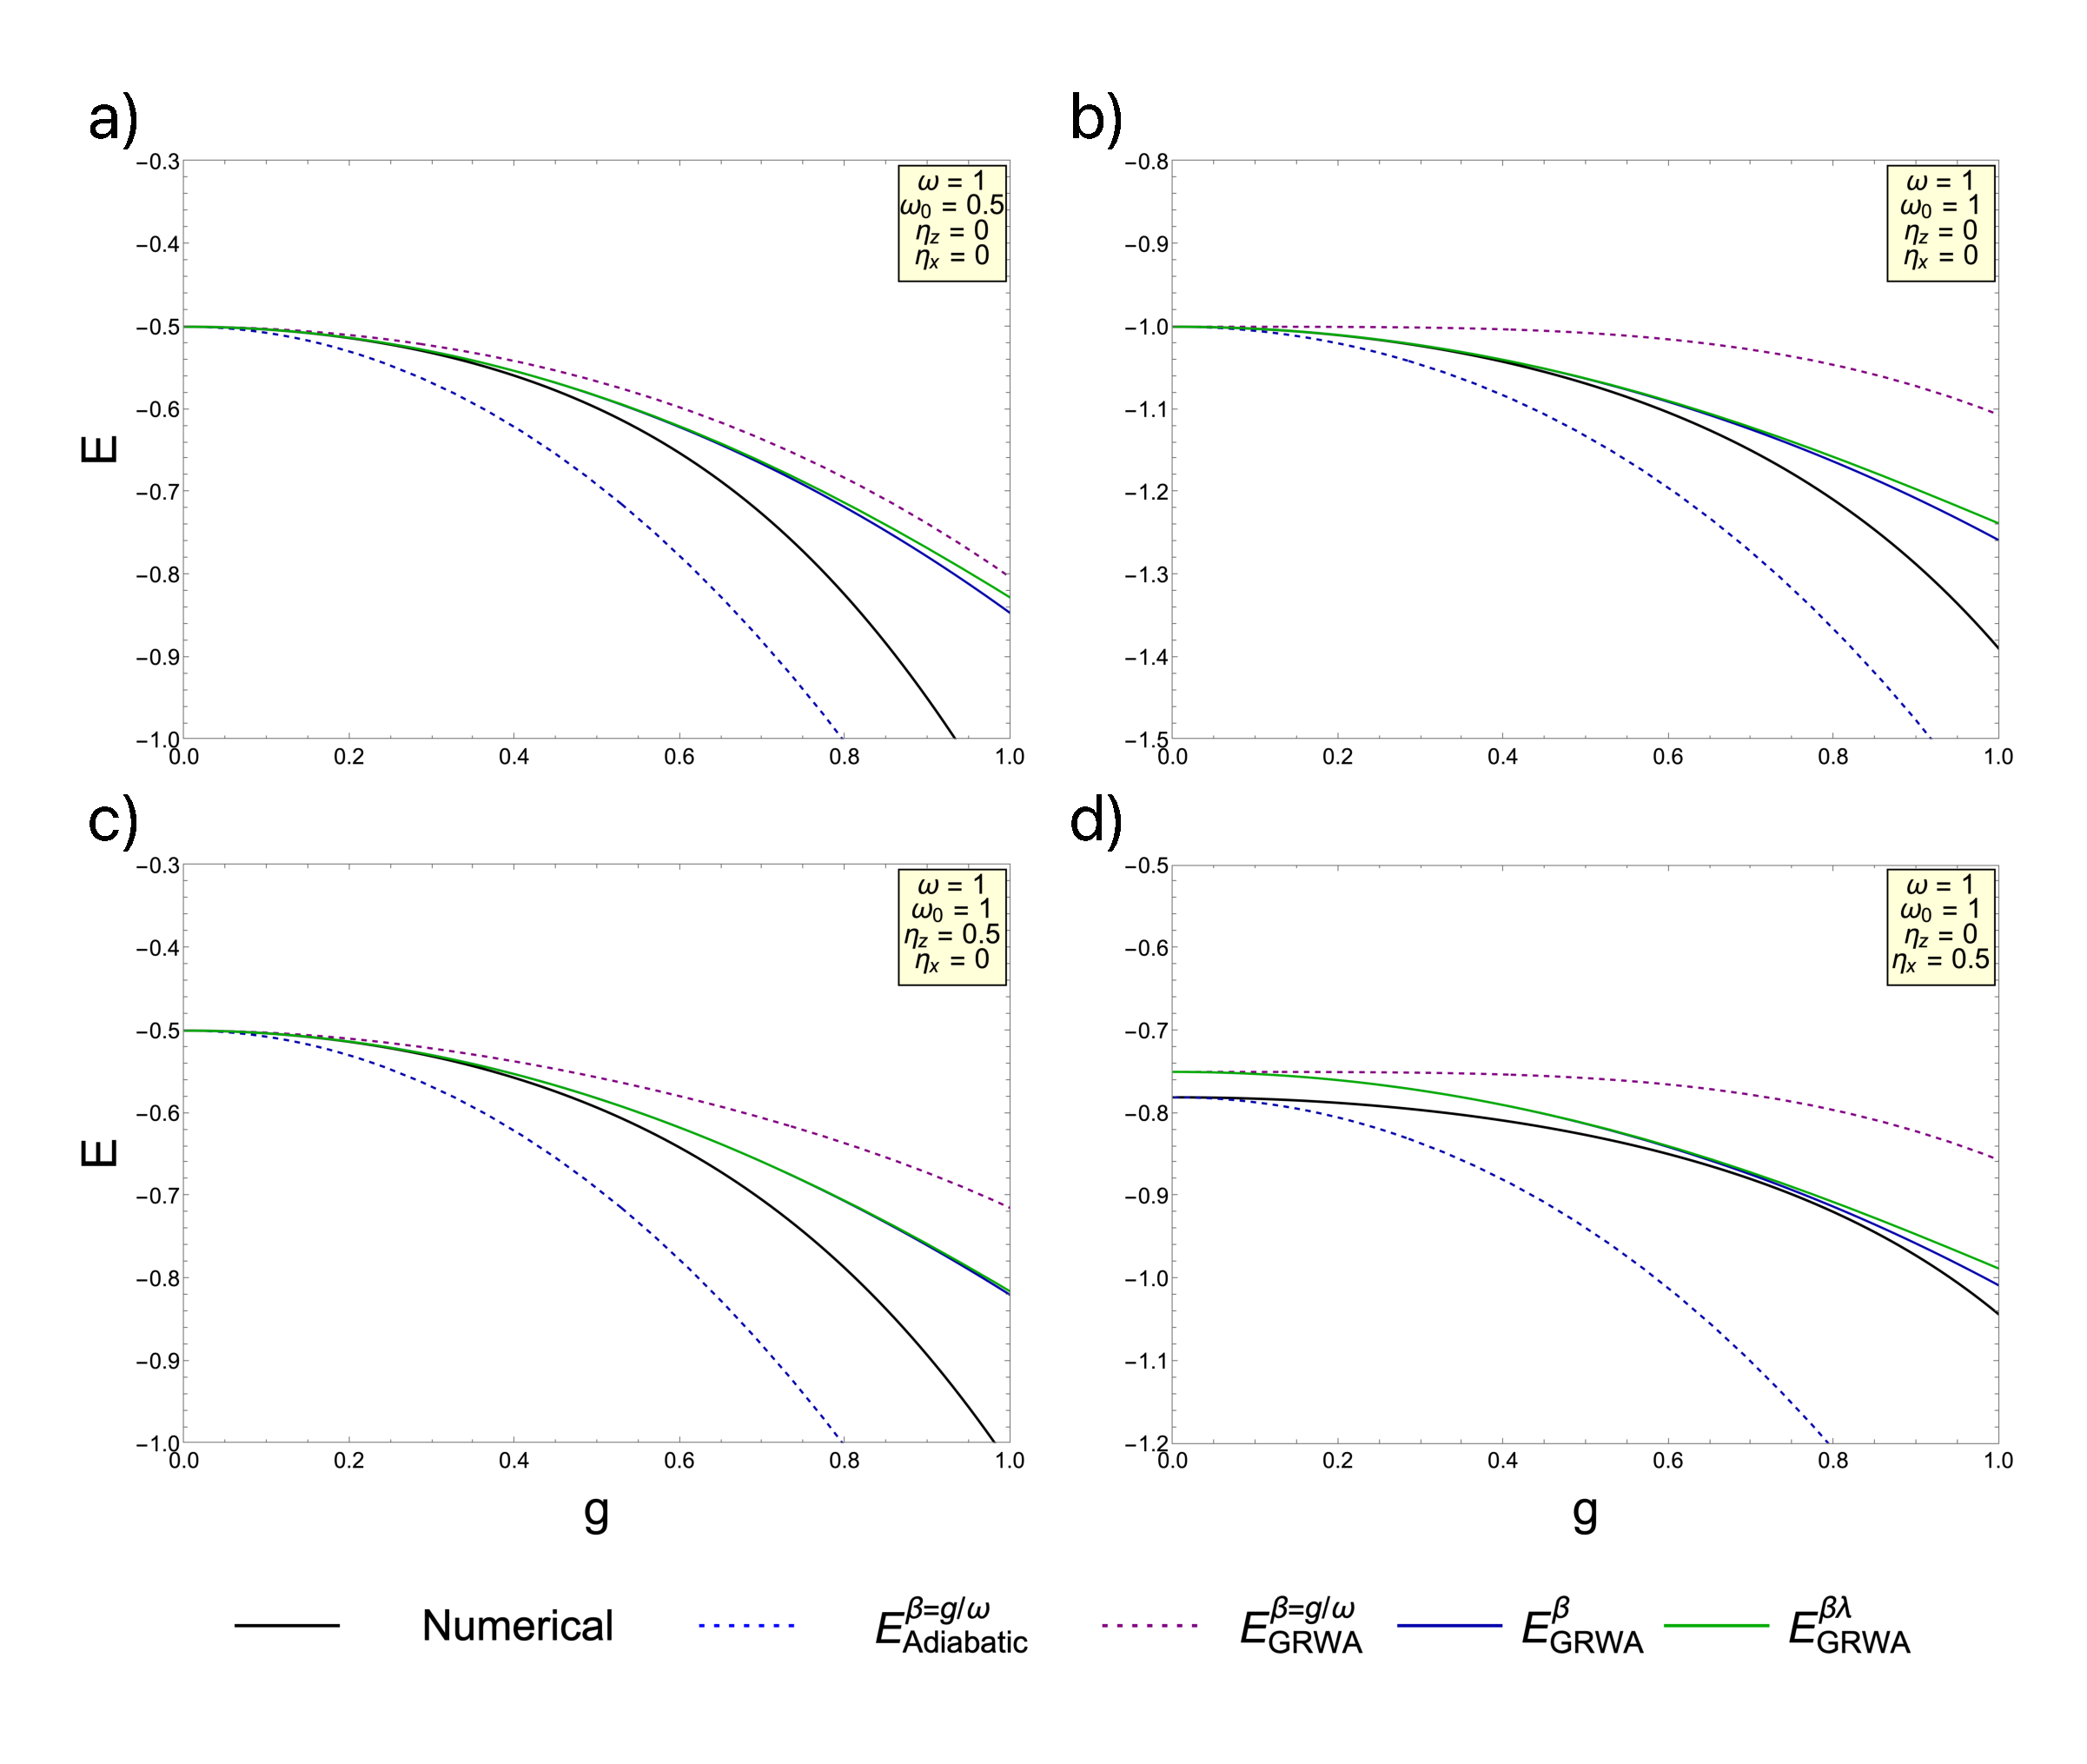
\includegraphics[width=0.95\linewidth]{Images APS v1/Estado Base.pdf}
    \caption{Energía del estado fundamental. El tratamiento variacional con $\beta$ (azul sólido) y $\beta + \lambda$ (verde sólido) muestra mejora sistemática sobre aproximaciones convencionales en todos los regímenes de acoplamiento.}
    \label{fig:Ground State}
\end{figure}

Para capturar correlaciones cuánticas adicionales, implementamos una transformación de squeezing $\hat{V} = \exp\left[{\lambda\left(\hat{a}^{2} - \hat{a}^{\dagger2}\right)}\right]$ que conduce a la expresión:

\begin{gather}
E_{\text{GRWA,GS}}^{\beta,\lambda} = \omega \sinh^{2}(2\lambda) - \omega_{0} e^{-\frac{\beta^{2}}{2} e^{-4\lambda}} + \frac{1}{2}\left[ (\omega\beta -2g)\beta + \eta_{x} + \frac{\eta_{z}}{2}\left( e^{-2\beta^{2}e^{-4\lambda}} +3 \right) \right].
\end{gather}

La optimización simultánea de ambos parámetros ($\partial E/\partial\beta = 0$, $\partial E/\partial\lambda = 0$) proporciona la descripción más precisa del estado fundamental. En el límite de acoplamiento débil, los parámetros admiten formas analíticas compactas:

\begin{gather}
\beta_{0} \simeq \frac{g}{\omega + \omega_{0}-\eta_{z}}, \qquad \lambda_{0} \simeq \frac{\omega_{0}-\eta_{z}}{2\omega} \left( \frac{g}{\omega + \omega_{0} -\eta_{z}} \right)^{2},
\end{gather}

revelando cómo las interacciones materiales modulan la compresión del campo.

\subsubsection{Valor medio del número de fotones}

El cálculo del número medio de fotones $\langle n \rangle = \langle a^{\dagger}a \rangle$ cuantifica el dressing del vacío inducido por el acoplamiento fuerte. Como muestra la Figura~\ref{fig:Expectation Value}, la GRWA aproxima el crecimiento de $\langle n \rangle$ con $g$, capturando tanto la tendencia cualitativa como las modificaciones introducidas por las interacciones materiales.

\begin{figure}[H]
    \centering
    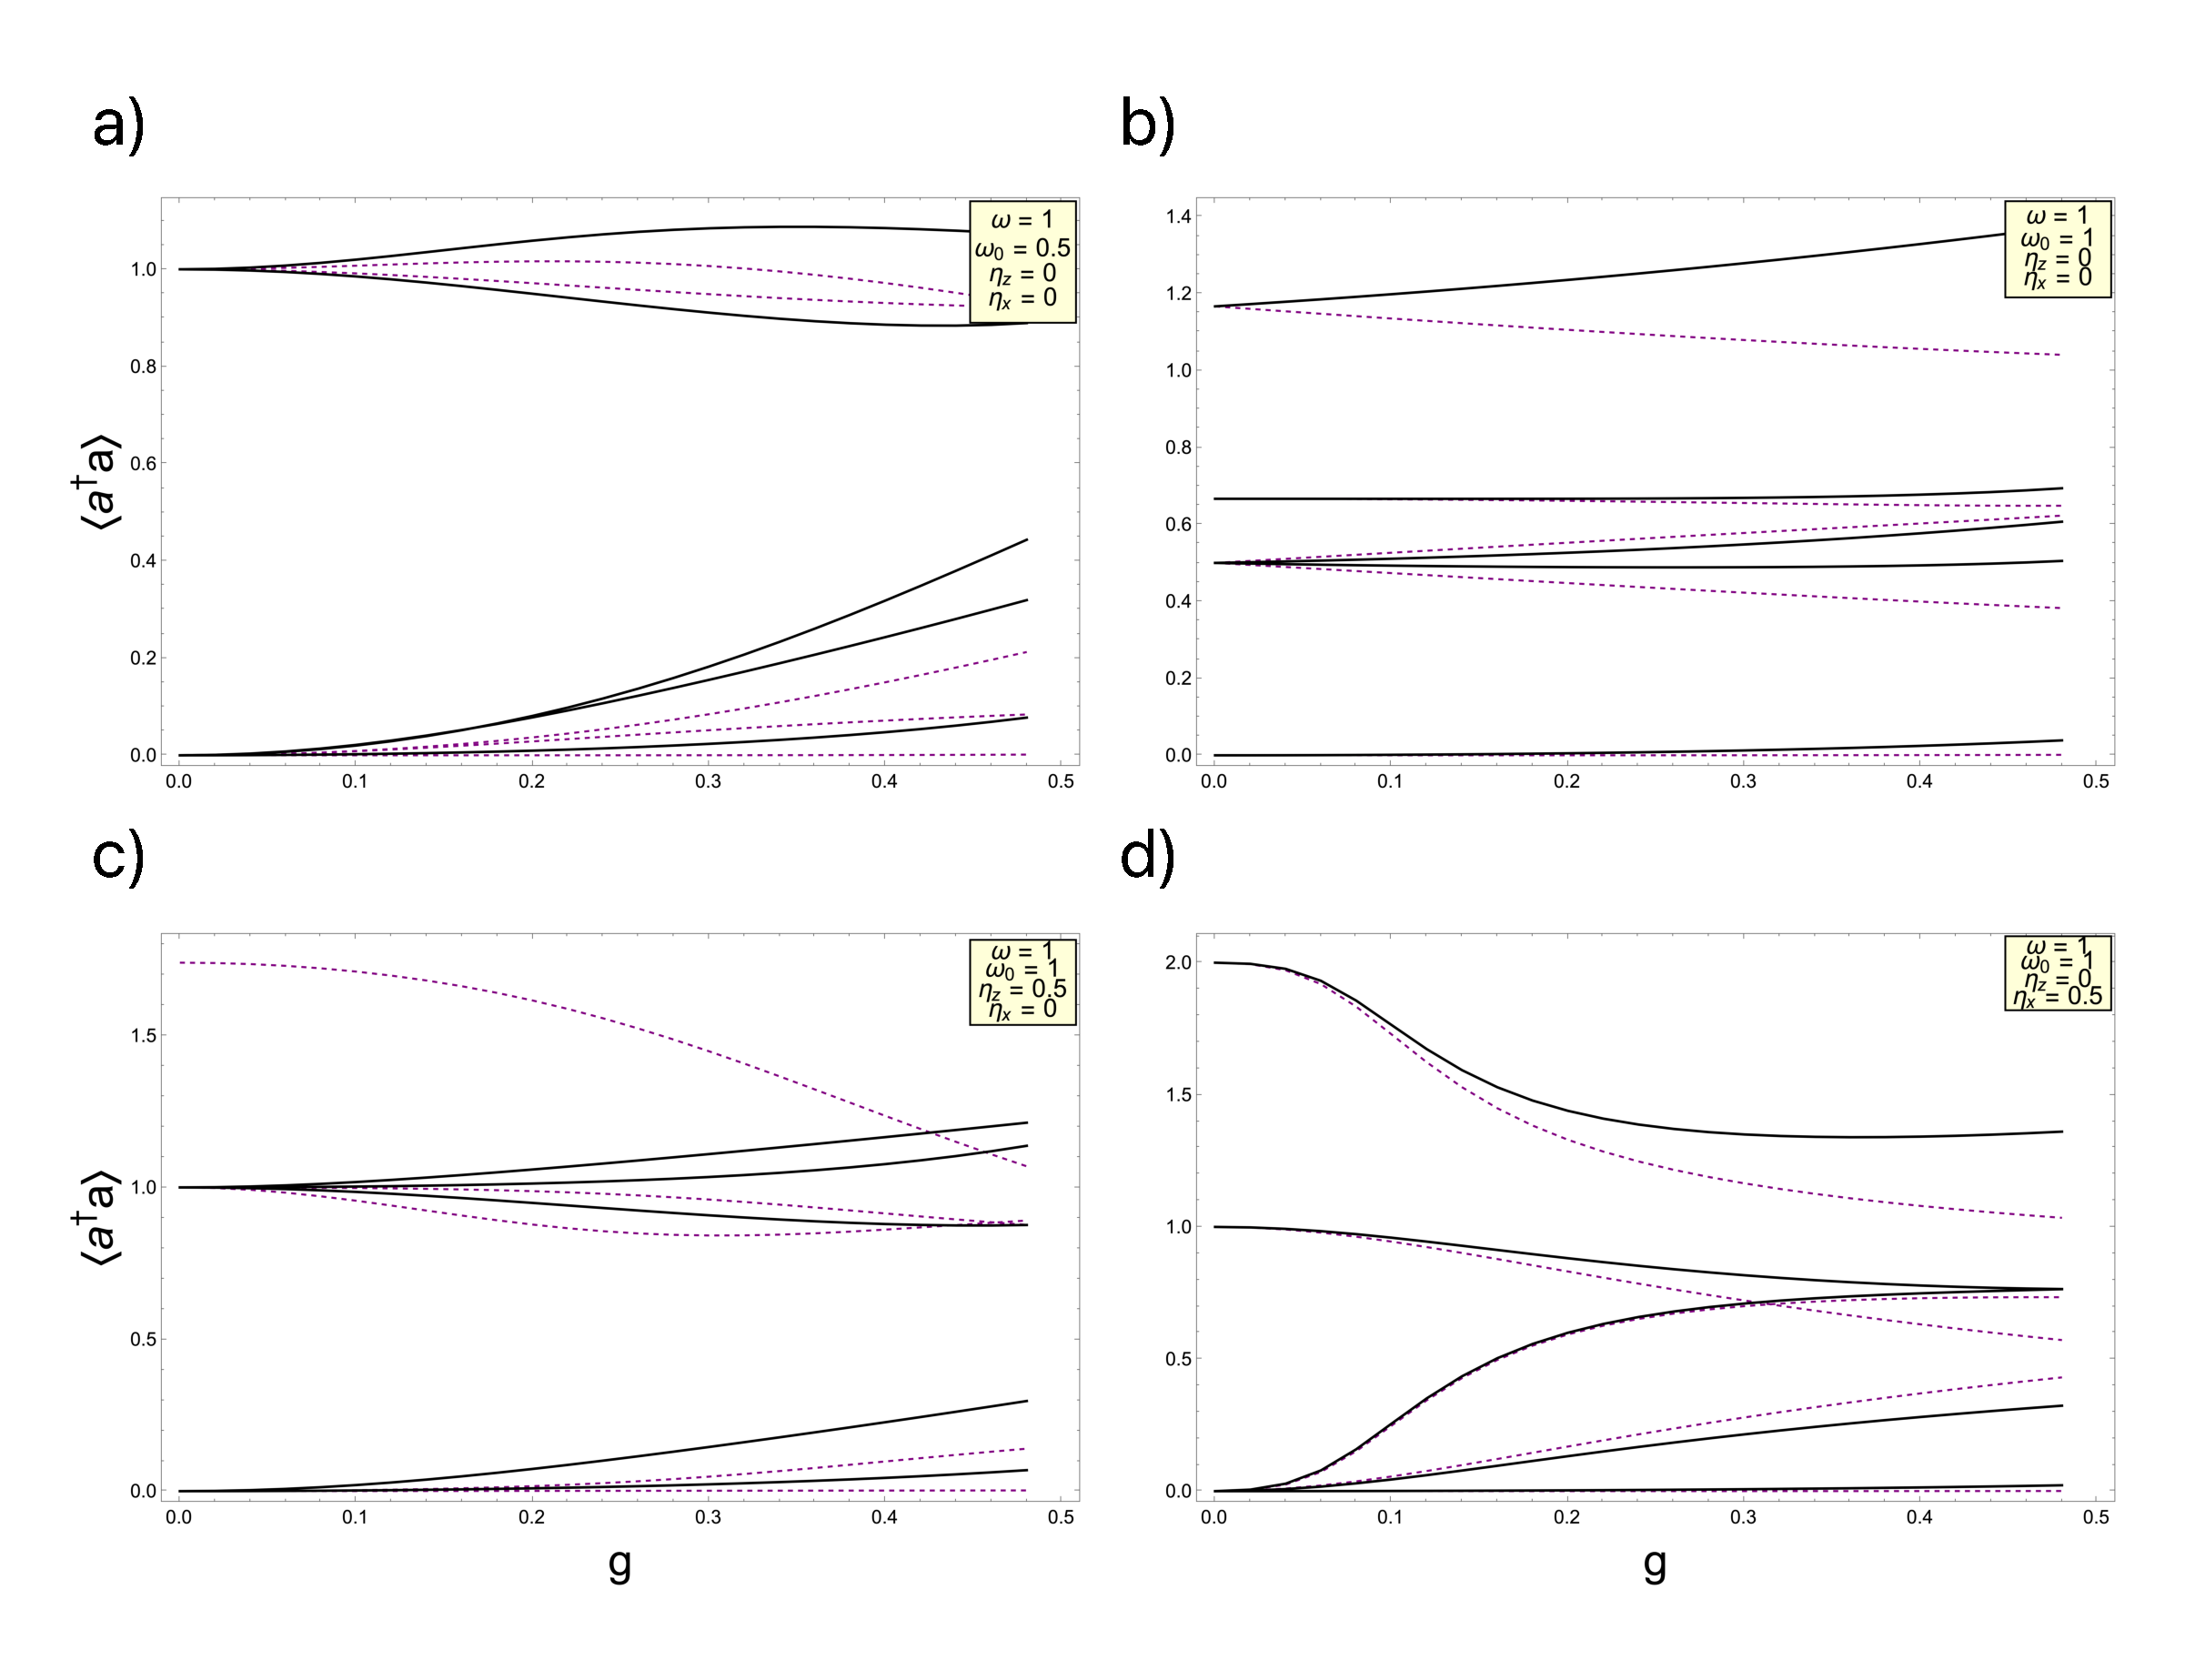
\includegraphics[width=0.95\linewidth]{Images APS v1/Promedio.pdf}
    \caption{Número medio de fotones en el estado fundamental. La GRWA captura el dressing fotónico inducido por el acoplamiento fuerte y la influencia diferenciada de las interacciones materiales.}
    \label{fig:Expectation Value}
\end{figure}

Observamos que $\eta_z$ acopla directamente con $\hat{J}_{z}$ y modifica significativamente el desplazamiento del oscilador, $\eta_x$ (asociado a procesos spin-flip) influye principalmente en la estructura del entrelazamiento y el espectro de excitaciones, sin afectar prominentemente el desplazamiento medio del campo. Esta distinción física emerge naturalmente de nuestro tratamiento variacional y constituye un insight valioso para el diseño de sistemas cuánticos con acoplamientos controlados.





%%%%%%%%%%%%%%%%%%%%%%%%%%%%%%
\subsection{Reproducción analítica de dinámicas no markovianas en átomos gigantes}
%%%%%%%%%%%%%%%%%%%%%%%%%%%%%%

He realizado una revisión y reproducción analítica de los métodos desarrollados en el artículo ``Non-Markovian dynamics of giant emitters beyond the Weisskopf-Wigner approximation''~\cite{gonzalez2025}, lo que me ha permitido dominar herramientas teóricas esenciales para el estudio de sistemas cuánticos abiertos con estructura espacial extendida.

He implementado sistemáticamente el formalismo exacto basado en la transformada de Laplace para resolver la dinámica de emisores cuánticos acoplados a guías de onda estructuradas. Logré reproducir la solución exacta para la amplitud de probabilidad del estado excitado:

\[\alpha(t) = \lim_{\epsilon\to 0}\int_{-\omega_{\max}}^{-\omega_{\min}}\frac{dy}{2\pi}\frac{J(-y)e^{iyt}}{[y+\Delta-iG(-\epsilon+iy)]\,[y+\Delta-iG(\epsilon+iy)]} + \sum_{j=\pm}r_{j}e^{-iy_{j}t}.\]

Esta descomposición revela físicamente la coexistencia de dos tipos de estados: estados de scattering dentro del continuo que eventualmente decaen, y estados ligados fuera del continuo (BOC) que persisten indefinidamente. La validación de este formalismo me ha permitido comprender en profundidad cómo las singularidades de van Hove en la función espectral $J(\omega) = \frac{2g_{0}^{2}}{\sqrt{4\xi^{2}-\omega^{2}}}$ modifican cualitativamente la dinámica de emisión espontánea.

%%%%%%%%%%%%%%%%%%%%%%%%%%%%%%
\subsubsection{Caracterización de estados ligados y efectos de localización}
%%%%%%%%%%%%%%%%%%%%%%%%%%%%%%

Un resultado clave que he verificado es la formación de estados ligados fotónicos localizados exponencialmente alrededor del emisor, con longitud de localización $\lambda_{\pm} = \cosh^{-1} (|y_{\pm}|/2\xi)$. Estos estados emergen cuando la frecuencia del emisor se sitúa cerca de los bordes de la banda fotónica, donde la aproximación markoviana deja de ser válida. 

La reproducción del perfil espacial del campo radiante en el estado estacionario:

\[\langle a_n^{\dagger}a_n \rangle_{\pm} = \frac{g_0^2 r_{\pm}^2}{y_{\pm}^2 - 4\xi^2} e^{-2\kappa_{\pm}|n|},\]

confirma cómo la excitación queda atrapada en la vecindad del emisor, un fenómeno fundamental para el confinamiento cuántico de luz.

%%%%%%%%%%%%%%%%%%%%%%%%%%%%%%
\subsubsection{Extensión a átomos gigantes y emergencia de BICs}
%%%%%%%%%%%%%%%%%%%%%%%%%%%%%%

He extendido exitosamente el formalismo al caso de átomos gigantes, donde el emisor se acopla en múltiples puntos espacialmente separados. Para el caso mínimo de $N_c=2$ puntos de acoplamiento, reproduje la modificación del acoplamiento efectivo:

\[\tilde{g}_k = \frac{g_0}{N_c\sqrt{N}} \frac{\sin(kdN_c/2)}{\sin(kd/2)},\]

que conduce a la función espectral efectiva $J_{\text{eff}}(\omega) = J(\omega) \mathcal{G}(\omega)$. Crucially, verifiqué la emergencia de estados ligados dentro del continuo (BIC) en frecuencias específicas $\omega_m = 2\xi\cos(\pi(2m+1)/d)$, donde la interferencia destructiva suprime completamente la emisión al continuo.



El dominio de estas herramientas me permite abordar el estudio de fenómenos colectivos en sistemas espín-bosón multimodo con acoplamiento fuerte. La comprensión de efectos no markovianos, estados ligados e interferencia en átomos gigantes constituye la base para extender estos conceptos a sistemas multiqubit y configuraciones de Dicke multimodo.

El formalismo de transformada de Laplace y la caracterización de funciones espectrales permitirán analizar sistemáticamente cómo la competencia entre acoplamiento fuerte, disipación y efectos de memoria modifica las transiciones de fase cuántica y genera nuevos estados estacionarios fuera del equilibrio.


%%%%%%%%%%%%%%%%%%%%%%%%%%%%%%
%%%%%%%%%%%%%%%%%%%%%%%%%%%%%%
\section{Bibliografía}
%%%%%%%%%%%%%%%%%%%%%%%%%%%%%%
%%%%%%%%%%%%%%%%%%%%%%%%%%%%%%

\printbibliography[heading=none]


%%%%%%%%%%%%%%%%%%%%%%%%%%%%%%
%%%%%%%%%%%%%%%%%%%%%%%%%%%%%%
\section{Calendario de actividades}
%%%%%%%%%%%%%%%%%%%%%%%%%%%%%%
%%%%%%%%%%%%%%%%%%%%%%%%%%%%%%

\begin{figure}[H]
    \centering
    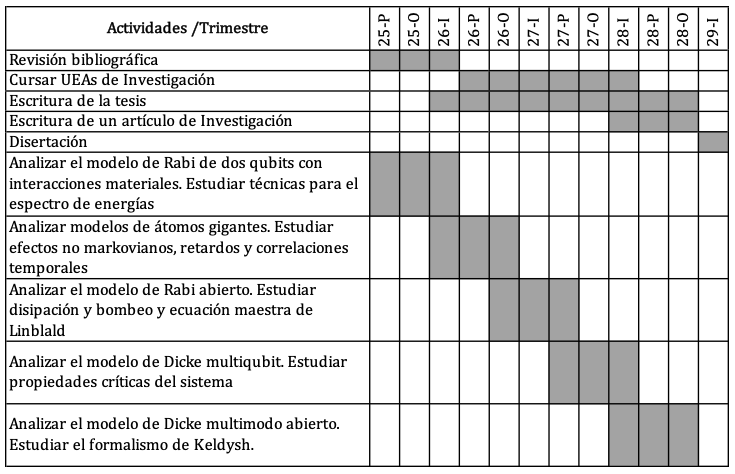
\includegraphics[width=1\linewidth]{Images/Calendario.png}
    \label{Calendario}
\end{figure}








\end{document}
